\begin{itemize}
\item Aufgrund der De Broglie-Wellenlänge haben Elektronen eine Wellenlänge, wenn sie einen Impuls besitzen.
\item Die Wellenlänge eines Elektron ist bei bestimmten Konfigurationen groß genug, dass Interferenzerscheinungen auftreten (Das Elektron \textbf{verhält} sich wie eine Welle, ist aber keine.)
\item Theoretisch lässt sich seinen Wellenlänge $\lambda$ durch das Gleichsetzen der Gleichung des Impulses $\vec{p}=m\cdot\vec{v}$ mit der Formel für den Photonenimpuls $\vec{p}=\frac{h}{\lambda}$:

$m\cdot\vec{v}=\frac{h}{\lambda}$ \tabto{0.5\textwidth} ; umstellen nach $\lambda$

$\lambda = \frac{h}{m \cdot v} $

\item Um die Geschwindigkeit $v$, bei einem Versuch mit Elektronenbeschleunigung durch ein elektrisches Feld, zu ersetzen, setzt man zunächst die Gleichungen der kinetischen Energie $E_{kin}$ mit der Gleichung der Elektrischen $E_{el}$ gleich und formt anschließend nach $v$ um.

$\frac{1}{2} m_e \cdot v^2 = e \cdot U_a$ \tabto{0.5\textwidth} ; $U_a$ ist die Beschleunigungsspannung, mit der das Elektron in dem jeweiligen Versuch beschleunigt wurde.

$v = \sqrt{\frac{2e \cdot U_a}{m_e}}$

durch Einsetzen folgt dann:

\Large $\lambda = \frac{h \sqrt{m_e}}{m \cdot \sqrt{2e \cdot U_a}} $
\end{itemize}

\subsection{...an Grafit}
\begin{itemize}
\item Da Elektronen demnach eine sehr kleine Wellenlänge haben, benutzt man oft Kristalle um Interferenzmuster zu erzeugen.
\item An den Netzebenen des Kristalls, in denen die Atome regelmäßig angeordnet sind, werden Elektronen, ähnlich wie Licht an dünnen Schichten (Glimmer), gestreut.
\item Auf dem Leuchtschirm der Röhre kommt es je nach Gangunterschied über die verschiedenen Netzebenen zu Maxima und Minima.
\item Wichtig: Bei Grafit haben die Atome in einer Ebene einen anderen Abstand d zu einander, als die Atome zwischen den Ebenen. Es gibt als zwei "Spaltabstände" und folglich auch zwei Maxima 1. (2.,...,n.) Ordnung.

\item Der Gangunterschied $\delta = 2d\cdot\sin{\alpha} $ für konstruktive Interferenz muss ein natürliches vielfaches der Wellenlänge $\lambda$ sein.

$n \cdot \lambda = 2d \cdot \sin{\alpha}$

\Large $\sin{\alpha} = \frac{n \cdot \lambda}{2d}$ Bragg'sche Bedingung / Gleichung
\end{itemize}

Achtung in der Zeichnung ist $\alpha$ mit $\Theta$ vertauscht!

\begin{figure}[h!]
\centering 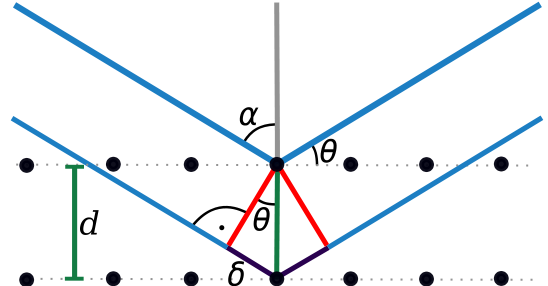
\includegraphics[width=0.8\textwidth]{Streuung_an_Graphit}
\caption{Abbildung von: \url{https://upload.wikimedia.org/wikipedia/commons/thumb/c/ca/Bragg.svg/548px-Bragg.svg.png}}
\end{figure}



\subsubsection{Versuch}
\begin{itemize}
\item Im Versuch wird ein Elektronenstrahl auf einen Graphitkristall geleitet, an diesem kommt es zu Streuung und es bilden sich jeweils zwei ringförmige Maxima auf dem Schirm.
\item Bezeichnet man den Abstand vom Maximum n. Ordnung zum Maximum 0. Ordnung mit $r$ und den Abstand vom Kristall zum Schirm mit $l$ folgt:

$\tan{2\alpha} = \frac{r}{l}$
\item Um die Wellenlänge der Elektronen experimentell zu bestimmen, setzten wir dies Formel mit der Bragg'schen Gleichung gleich.

$2\sin{\alpha} = tan{2\alpha}$

wendet man die Kleinwinkelnäherung an, folgt: \\
\Large $\frac{n\cdot\lambda}{2d}=\frac{r}{l}$

\normalsize

umgestellt nach $\lambda$:\\
\Large $\lambda = \frac{2dr}{n\cdot l}$

\normalsize

ohne Winkelnäherung:\\
\Large $2\cdot\arcsin(\frac{n\cdot \lambda}{2d})=\arctan(\frac{r}{l}) $

\Large $\arcsin(\frac{n\cdot \lambda}{2d})=\frac{1}{2}\cdot\arctan(\frac{r}{l})$ 

\Large $\frac{n\cdot \lambda}{2d}=\sin(\frac{1}{2}\cdot\arctan(\frac{r}{l}))$ 

\Large $\lambda=\sin(\frac{1}{2}\cdot\arctan(\frac{r}{l}))\cdot 2d \cdot \frac{1}{n}$ \tabto{0.5\textwidth} ; meistens ist n=1 

\normalsize

\item Nice to know: Es kommt nur zur Interferenz, wenn die Bragg'sche Gleichung erfüllt ist. Dafür muss $\alpha$, für eine bestimmte Wellenlänge, auch eine bestimmte Größe haben. Im Experiment wird deshalb eine Graphitfolie benutzt, auf der die Kristallgitter in den verschiedensten Anordnungen liegen. So ist statistisch gesehen immer ein Kristall im richtigen Winkel zum Elektronenstrahl.
\end{itemize}

\subsection{...am Doppelstpalt}
\begin{itemize}
\item Grundsätzlich gelten die gleichen Formeln wie bei Interferenz mit Licht. Allerdings muss der Spaltabstand $d$, aufgrund der ebenfalls sehr kleinen Wellenlängen, sehr klein sein, um überhaupt ein Interferenzmuster detektieren zu kommen.\\
Das Interferenz Muster ist so klein, dass man es nur mit einem Elektronenmikroskop sichtbar machen kann.
\item Bedingungen für konstruktive Interferenz: $\delta = n \cdot \lambda$\\
für destruktive Interferenz: $\delta = (n-\frac{1}{2}) \cdot \lambda$
\end{itemize}

\subsubsection{Versuch}
\begin{itemize}
\item Um die Wellenlänge $\lambda$ experimentell herauszufinden, gilt, wenn $d$ der Spaltabstand ist, $a$ der Abstand zum Schirm und $d_k$ der Abstand des k. Maximum zum 0. Maximum ist:

$\tan{\alpha}=\frac{d_k}{a}$ und $\sin{\alpha}=\frac{k \cdot\lambda}{d}$

Dann entweder durch Kleinwinkelnäherung:\\
\Large $\lambda = \frac{d_k \cdot d}{k \cdot a}$

\normalsize oder ohne:

\Large $\lambda = \sin(\arctan(\frac{d_k}{a})) \cdot \frac{d}{k}$
\end{itemize}